\documentclass[handout, 11pt]{beamer}
\mode
<presentation>{\usetheme{Madrid}}
\institute[UF]{\inst{1}
University of Florida\\
Department of Finance, Insurance, and Real Estate}
\usepackage{adjustbox}
\usepackage{tikz}
\usetikzlibrary{positioning}
\usetikzlibrary{positioning}
\usetikzlibrary{positioning}
\usetikzlibrary{positioning}
\usetikzlibrary{positioning}
\usetikzlibrary{positioning}
\usetikzlibrary{positioning}
\usetikzlibrary{positioning}
\usetikzlibrary{positioning}
\usetikzlibrary{positioning}
\usetikzlibrary{positioning}
\usetikzlibrary{positioning}
\usetikzlibrary{positioning}
\usetikzlibrary{positioning}
\usetikzlibrary{positioning}
\definecolor{darkgreen}{RGB}{31,156,17}
\usepackage{booktabs}
\setbeamertemplate{headline}{\begin{beamercolorbox}[ht=2.25ex, dp=3.75ex]{section in head/foot}
\insertnavigation{\paperwidth}
\end{beamercolorbox}}
\AtBeginSection{\begin{frame}
\frametitle{Table of Contents}
\tableofcontents[currentsection]
\end{frame}}
\begin{document}
\title[MC Sim]{Monte Carlo Simulation}
\subtitle{Analyzing Probabilities of Outputs}
\author[DeRobertis]{Nick DeRobertis\inst{1}}
\date{\today}
\begin{frame}
\titlepage
\label{title-frame}
\end{frame}
\begin{section}{Introduction}
\begin{frame}
\frametitle{What is Monte Carlo Simulation?}
\begin{columns}
\begin{column}{0.5\textwidth}
\vbox to 0.8\textheight{\begin{itemize}
\item \textbf{Monte Carlo Simulation}
is a technique which allows understanding the probability of acheiving certain outputs from a model.
\vfill
\item This gives the modeler a greater understanding of the likelihood of different outputs, rather than relying on a single number
\end{itemize}}
\end{column}
\begin{column}{0.5\textwidth}
\vbox to 0.8\textheight{\centering
\vfill
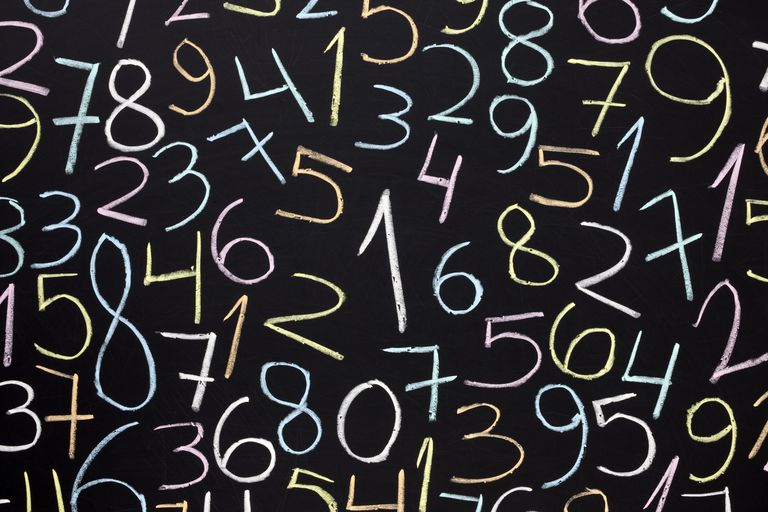
\includegraphics[height=1.0\textheight, keepaspectratio, width=0.9\textwidth]{Sources/random-numbers.jpg}
\vfill
\vfill}
\end{column}
\end{columns}
\end{frame}
\begin{frame}
\frametitle{Why Use Monte Carlo Simulation?}
\begin{itemize}
\item Imagine you have a one-time opportunity to place a bet for \$1. 
\vfill
\item If you win the bet, you will receive \$2. If you lose the bet, you will lose \$750,000. You cannot avoid the payment by declaring bankruptcy.
\vfill
\item The odds of winning the bet are 999,999/1,000,000. In 1/1,000,000 you lose the \$750,000.
\vfill
\item The expected profit from the bet is \$0.25. Should you take it? Depends on your risk tolerance.
\vfill
\item Therefore not only the expected outcome matters, but also what other outcomes may occur and their probabilities.
\end{itemize}
\end{frame}
\begin{frame}
\frametitle{Monte Carlo Simulation in One Picture}
\begin{center}
\begin{adjustbox}{width=0.9\textwidth, height=0.8\textheight, keepaspectratio}
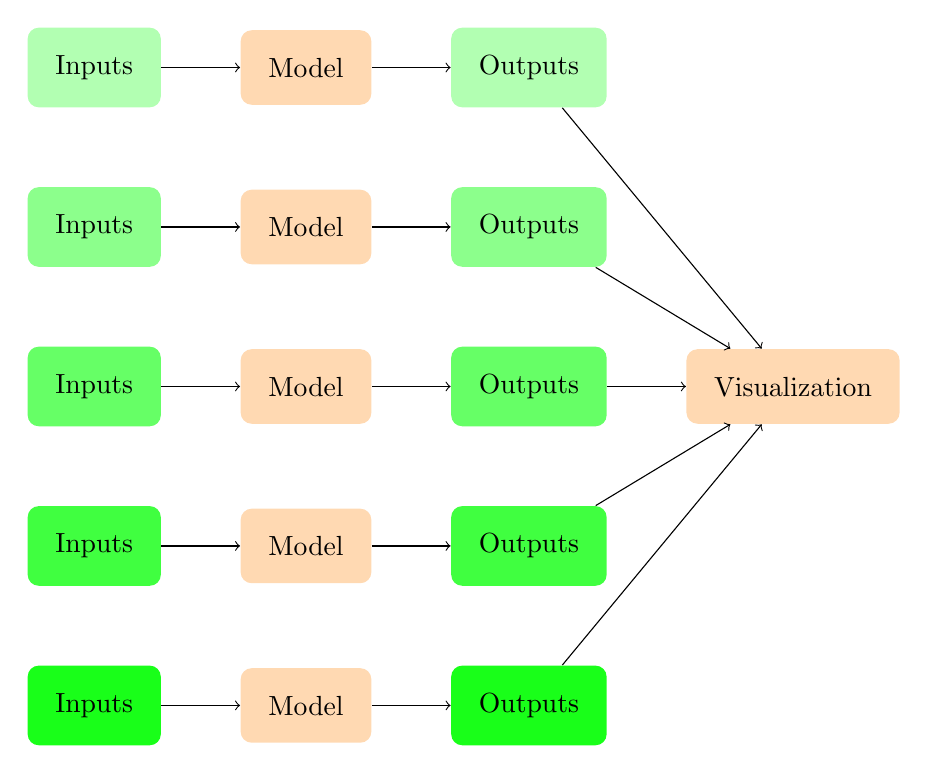
\begin{tikzpicture}
\node [fill=green!30, rounded corners, inner sep=10pt] (b200bda0-72d2-4648-b249-303eddddc010)  {Inputs};
\node [fill=orange!30, rounded corners, inner sep=10pt, right=of b200bda0-72d2-4648-b249-303eddddc010] (b694cda5-d108-4fdc-83e0-c2210708c0fd)  {Model};
\node [fill=green!30, rounded corners, inner sep=10pt, right=of b694cda5-d108-4fdc-83e0-c2210708c0fd] (3b75faa6-8038-497f-8bef-f7b74f3d13a3)  {Outputs};
\path [draw, ->] (b200bda0-72d2-4648-b249-303eddddc010) -- (b694cda5-d108-4fdc-83e0-c2210708c0fd);
\path [draw, ->] (b694cda5-d108-4fdc-83e0-c2210708c0fd) -- (3b75faa6-8038-497f-8bef-f7b74f3d13a3);
\node [fill=green!45, rounded corners, inner sep=10pt, below=of b200bda0-72d2-4648-b249-303eddddc010] (7ea26fa0-5c3f-40a2-a00d-35336c746af3)  {Inputs};
\node [fill=orange!30, rounded corners, inner sep=10pt, right=of 7ea26fa0-5c3f-40a2-a00d-35336c746af3] (0b50a846-3830-491f-8a23-6fe38100fde2)  {Model};
\node [fill=green!45, rounded corners, inner sep=10pt, right=of 0b50a846-3830-491f-8a23-6fe38100fde2] (7de8f427-da5d-42e8-9d67-7531a82cae41)  {Outputs};
\path [draw, ->] (7ea26fa0-5c3f-40a2-a00d-35336c746af3) -- (0b50a846-3830-491f-8a23-6fe38100fde2);
\path [draw, ->] (0b50a846-3830-491f-8a23-6fe38100fde2) -- (7de8f427-da5d-42e8-9d67-7531a82cae41);
\node [fill=green!60, rounded corners, inner sep=10pt, below=of 7ea26fa0-5c3f-40a2-a00d-35336c746af3] (17027155-7cbd-475a-bc0e-e9d828aa626a)  {Inputs};
\node [fill=orange!30, rounded corners, inner sep=10pt, right=of 17027155-7cbd-475a-bc0e-e9d828aa626a] (382f848a-b7e4-4bfa-a11e-b7afa45ef15e)  {Model};
\node [fill=green!60, rounded corners, inner sep=10pt, right=of 382f848a-b7e4-4bfa-a11e-b7afa45ef15e] (a3c31892-b05f-453b-8ac2-c6f78dd06fee)  {Outputs};
\path [draw, ->] (17027155-7cbd-475a-bc0e-e9d828aa626a) -- (382f848a-b7e4-4bfa-a11e-b7afa45ef15e);
\path [draw, ->] (382f848a-b7e4-4bfa-a11e-b7afa45ef15e) -- (a3c31892-b05f-453b-8ac2-c6f78dd06fee);
\node [fill=green!75, rounded corners, inner sep=10pt, below=of 17027155-7cbd-475a-bc0e-e9d828aa626a] (8fbf7476-c680-4c99-9890-b9b9e7096022)  {Inputs};
\node [fill=orange!30, rounded corners, inner sep=10pt, right=of 8fbf7476-c680-4c99-9890-b9b9e7096022] (e70c9f21-5080-46e1-8893-5a615b36a7b8)  {Model};
\node [fill=green!75, rounded corners, inner sep=10pt, right=of e70c9f21-5080-46e1-8893-5a615b36a7b8] (913fa5e6-a1fa-4059-bc2b-7a840e562e2a)  {Outputs};
\path [draw, ->] (8fbf7476-c680-4c99-9890-b9b9e7096022) -- (e70c9f21-5080-46e1-8893-5a615b36a7b8);
\path [draw, ->] (e70c9f21-5080-46e1-8893-5a615b36a7b8) -- (913fa5e6-a1fa-4059-bc2b-7a840e562e2a);
\node [fill=green!90, rounded corners, inner sep=10pt, below=of 8fbf7476-c680-4c99-9890-b9b9e7096022] (384abb2e-47d8-4eb9-84c8-d03a6e398f38)  {Inputs};
\node [fill=orange!30, rounded corners, inner sep=10pt, right=of 384abb2e-47d8-4eb9-84c8-d03a6e398f38] (9b47db5b-44c7-4734-9e60-ff14b55ccea0)  {Model};
\node [fill=green!90, rounded corners, inner sep=10pt, right=of 9b47db5b-44c7-4734-9e60-ff14b55ccea0] (c9bc5e25-bcb5-4352-9e98-84cbf631c29f)  {Outputs};
\path [draw, ->] (384abb2e-47d8-4eb9-84c8-d03a6e398f38) -- (9b47db5b-44c7-4734-9e60-ff14b55ccea0);
\path [draw, ->] (9b47db5b-44c7-4734-9e60-ff14b55ccea0) -- (c9bc5e25-bcb5-4352-9e98-84cbf631c29f);
\node [fill=orange!30, rounded corners, inner sep=10pt, right=of a3c31892-b05f-453b-8ac2-c6f78dd06fee] (86a7d3e1-4f96-4cd2-a492-e799da50694f)  {Visualization};
\path [draw, ->] (3b75faa6-8038-497f-8bef-f7b74f3d13a3) -- (86a7d3e1-4f96-4cd2-a492-e799da50694f);
\path [draw, ->] (7de8f427-da5d-42e8-9d67-7531a82cae41) -- (86a7d3e1-4f96-4cd2-a492-e799da50694f);
\path [draw, ->] (a3c31892-b05f-453b-8ac2-c6f78dd06fee) -- (86a7d3e1-4f96-4cd2-a492-e799da50694f);
\path [draw, ->] (913fa5e6-a1fa-4059-bc2b-7a840e562e2a) -- (86a7d3e1-4f96-4cd2-a492-e799da50694f);
\path [draw, ->] (c9bc5e25-bcb5-4352-9e98-84cbf631c29f) -- (86a7d3e1-4f96-4cd2-a492-e799da50694f);
\end{tikzpicture}
\end{adjustbox}
\end{center}
\end{frame}
\begin{frame}
\frametitle{Basic Process for Monte Carlo Simulation}
\begin{itemize}
\item Monte Carlo simulation is carried out similarly to external scenario analysis.
\vfill
\item The main difference is that we manually picked specific cases for the inputs with scenario analysis.
\vfill
\item In Monte Carlo simulation, we assign distributions to the inputs, and input values are drawn from the distributions for each run of the model
\vfill
\item Finally, we can fit a probability distribution to the outputs to be able to talk about the chance of a certain outcome occurring
\end{itemize}
\end{frame}
\end{section}
\begin{section}[Run MC]{Running a First Monte Carlo Simulation}
\begin{frame}
\frametitle{Running Monte Carlo Simulations - Python or Excel?}
\begin{itemize}
\item Monte Carlo simulation can be applied to any model
\vfill
\item It is generally easier to run them in Python than in Excel.
\vfill
\item With pure Excel, you're either going to VBA or hacking something with data tables
\vfill
\item In Python, just loop for N iterations, each time drawing inputs, running the model, and collecting outputs.
\vfill
\item We will start with a pure Python model, then move to using
\texttt{xlwings}
to add Monte Carlo simulations to our Excel models.
\end{itemize}
\end{frame}
\begin{frame}
\frametitle{An Example Application}
\begin{block}{An Investment Problem}
You have \$1,000 now and need to pay \$1,050 in one year. You have available to you two assets: a risk free asset that returns 3\%, and a stock that returns 10\% with a 20\% standard deviation. How much should you invest in the two assets to maximize your probability of having at least \$1,050 in one year?
\end{block}
\vfill
\begin{itemize}
\item We must first construct the basic model which gets the portfolio value for given returns
\item Then draw values of the stock return from a normal distribution, and run the model many times and visualize the outputs. 
\item Then repeat this process with each weight to determine the best weight.
\end{itemize}
\end{frame}
\begin{frame}
\frametitle{Simluating Portfolio Values}
{
\setbeamercolor{block title}{bg=darkgreen}
\begin{block}{Example for Simulating Portfolio Values}
\begin{itemize}
\item Go to Canvas and download the Jupyter notebook "MC Investment Returns.ipynb" from Examples > Monte Carlo
\item I will go through this example notebook to solve the problem from the prior slide.
\end{itemize}
\end{block}
}
\end{frame}
\footnotesize
\begin{frame}
\frametitle{Intro Monte Carlo Lab, Level 1}
{
\setbeamercolor{block title}{bg=violet}
\begin{block}{Monte Carlo Simulation of DDM, Level 1}
\begin{enumerate}
\item You are trying to determine the value of a mature company. The company has had stable dividend growth for a long time so you select the dividend discount model (DDM).
\item $P = \frac{d_1}{r_s - g}$
\item The next dividend will be \$1, and your baseline estimates of the cost of capital and growth are 9\% and 4\%, respectively
\item Write a function which is able to get the price based on values of the inputs
\item Then you are concerned about mis-estimation of the inputs and how it could affect the price. So then assume that the growth rate has a mean of 4\% but a standard deviation of 1\%
\item Visualize and summarize the resulting probability distribution of the price
\end{enumerate}
\vfill
\begin{tabular*}{\textwidth}{@{\extracolsep{\fill}}ccc}
\toprule
\hfill & Level 2: Slide \textcolor{blue}{\underline{\ref{labs:intro-monte-carlo-lab-2}}} & \hfill\\

\end{tabular*}
\end{block}
}
\label{labs:intro-monte-carlo-lab-1}
\end{frame}
\normalsize
\end{section}
\begin{section}[Formal MC]{A More Formal Treatment of Monte Carlo Simulation}
\begin{frame}
\frametitle{Monte Carlo Simulation Process}
\footnotesize
For the model given by:
\begin{equation}
	y = f(X)
\end{equation}
\begin{equation}
	X = [x_1, x_2, ..., x_n]
\end{equation}
\begin{itemize}
\item $y:$
Model output
\item $X:$
Model input matrix
\item $x_i:$
Value of $i$th $x$ variable
\end{itemize}
To run $N$ Monte Carlo simulations, follow the following steps:
\begin{enumerate}
\item Assign a probability distribution for each
$x_i$
\item For each
$x_i$
randomly pick a value from its probability distribution. Store them as
$X_j$
\item Repeat the previous step $N$ times, yielding
$[X_1, X_2, ..., X_N]$
\item For each
$X_j$
calculate
$y_j = f(X_j)$
\item Store the values of
$X_j$
mapped to
$y_j$
\item Visualize and analyze
$y_j$
versus
$X_j$
\end{enumerate}
\end{frame}
\begin{frame}
\frametitle{Outputs from Monte Carlo Simulation}
\begin{itemize}
\item There are a multitude of outputs we can get from a Monte Carlo simulation. We saw a few already in the example.
\vfill
\item \textbf{Outcome probability distributions}
are the main output. We saw this with two approaches in the example, a
\underline{histogram}
and a
\underline{probability table.}
\vfill
\item We also examined the
\textbf{probability of a certain outcome}
in whether we reached the desired cash.
\vfill
\item The last main output is examining the
\textbf{relationship between inputs and outputs.}
for which common approaches include
\underline{scatter plots}
and
\underline{regressions.}
\end{itemize}
\end{frame}
\begin{frame}
\frametitle{Outcome Probability Distributions}
\begin{columns}
\begin{column}{0.5\textwidth}
\vbox to 0.8\textheight{\centering
\vfill
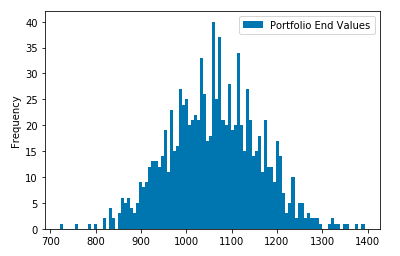
\includegraphics[height=0.4\textheight, keepaspectratio, width=0.9\textwidth]{Sources/outcome-probability-distribution.png}
\vfill
\begin{tabular}{c|c}
\multicolumn{2}{c}{Probability Table}\\

\toprule
Probability & Value\\

\cmidrule(lr){1-2}
25\% & 1020\\
50\% & 1039\\
75\% & 1053\\

\bottomrule
\end{tabular}
\vfill
\vfill}
\end{column}
\begin{column}{0.5\textwidth}
\vbox to 0.8\textheight{\begin{itemize}
\small
\vfill
\item The outcome probability distribution represents the chance of receiving different outcomes from your model.
\vfill
\item There are two main ways to visualize a probability distribution: a plot and a table.
\vfill
\item The plot, usually a
\underline{histogram}
or
\underline{KDE}
gives a high-level overview of the probabilities and can uncover any non-normal features of the distribution.
\vfill
\item The probability table represents the chance of receiving the given value or lower.
\end{itemize}}
\end{column}
\end{columns}
\end{frame}
\begin{frame}
\frametitle{Probability of a Certain Outcome - A Simple Example}
\begin{columns}
\begin{column}{0.5\textwidth}
\vbox to 0.8\textheight{\begin{itemize}
\item Imagine a box which contains red and blue balls. You do not know in advance how many there are of each color.
\vfill
\item You want to estimate the probability of getting a blue ball when pulling a ball from the box.
\vfill
\item To evaluate this, you grab a ball, write down its color, and put it back, 1,000 times.
\vfill
\item You pull a blue ball in 350 out of the 1,000 trials. What is the probability of getting blue?
\end{itemize}}
\end{column}
\begin{column}{0.5\textwidth}
\vbox to 0.8\textheight{\centering
\vfill
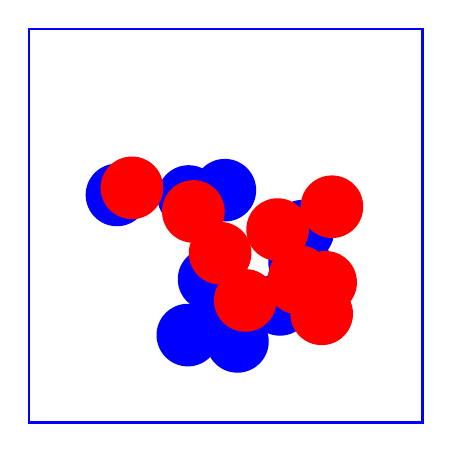
\begin{tikzpicture}
\coordinate [blue, thick, minimum width=5cm, minimum height=5cm, rectangle, draw] (1667a9cc-848a-4675-9f62-c78daa856976) at (0, 0) {};
\coordinate [fill, circle, inner sep=8pt, blue] (645a1077-2a88-4afa-af21-38ab3d5dad7d) at (0.69, -1.0) {};
\coordinate [fill, circle, inner sep=8pt, blue] (3acc752e-0aad-49bf-bc24-76fdb6b56ab1) at (-0.47, 0.37) {};
\coordinate [fill, circle, inner sep=8pt, blue] (c3d58977-b7cf-45f2-b7fb-8b2de6b2b41b) at (-0.48, -1.39) {};
\coordinate [fill, circle, inner sep=8pt, blue] (49170050-d004-42da-814a-84c7c58c1e31) at (-0.21, -0.68) {};
\coordinate [fill, circle, inner sep=8pt, blue] (51fca83a-3b5b-4e7c-a5ff-de1e4b60755d) at (-0.01, 0.45) {};
\coordinate [fill, circle, inner sep=8pt, blue] (7854f2fb-f403-4d24-b3a6-b6133a4ad1cb) at (0.98, -0.07) {};
\coordinate [fill, circle, inner sep=8pt, blue] (2034fbe1-22a1-4f80-9b54-e758564ac2c3) at (-1.38, 0.39) {};
\coordinate [fill, circle, inner sep=8pt, blue] (e6df66c1-12de-49ee-933d-4de44cc4ed6a) at (0.94, -0.47) {};
\coordinate [fill, circle, inner sep=8pt, blue] (8fe197b4-2a19-4c68-b29d-77606584eb06) at (0.15, -1.47) {};
\coordinate [fill, circle, inner sep=8pt, blue] (0bdc3333-1a57-43e1-a419-13228c44fd35) at (0.02, -1.26) {};
\coordinate [fill, circle, inner sep=8pt, red] (1aba35a1-0d28-47c4-bfec-5d97db2b157d) at (1.35, 0.24) {};
\coordinate [fill, circle, inner sep=8pt, red] (37459c04-9e05-4cc0-a4c3-c59c8785703b) at (-0.07, -0.35) {};
\coordinate [fill, circle, inner sep=8pt, red] (c843d684-68b4-46ee-80a7-e0d908fefb75) at (0.94, -0.65) {};
\coordinate [fill, circle, inner sep=8pt, red] (11ffb37b-ff47-47a3-b706-6c1adde1cb4a) at (-1.19, 0.48) {};
\coordinate [fill, circle, inner sep=8pt, red] (d23a5639-0239-4fc3-95c9-bd9a23098b7f) at (-0.41, 0.18) {};
\coordinate [fill, circle, inner sep=8pt, red] (dff8a69e-27b9-45b1-a0c3-6c329a9adb3c) at (0.92, -0.73) {};
\coordinate [fill, circle, inner sep=8pt, red] (415066e8-52f0-447c-af9d-362e244abca5) at (0.25, -0.95) {};
\coordinate [fill, circle, inner sep=8pt, red] (1fc342d3-2173-4067-ac2b-7a3943d3db42) at (0.66, -0.05) {};
\coordinate [fill, circle, inner sep=8pt, red] (58bc8ace-85db-47c1-ac25-be7af770b381) at (1.22, -1.12) {};
\coordinate [fill, circle, inner sep=8pt, red] (b4d4f131-cd20-466c-ac02-d54ff7b4ae13) at (1.27, -0.72) {};
\end{tikzpicture}
\vfill
\vfill}
\end{column}
\end{columns}
\end{frame}
\begin{frame}
\frametitle{Probability of a Certain Outcome, Formally}
\begin{itemize}
\item We followed the same logic when estimating the probability of receiving our desired cash in the investment example.
\vfill
\item $p = \frac{\text{Count of positive outcomes}}{\text{Count of trials}}$
\vfill
\item For the balls example, this is simply
$p = \frac{350}{1000} = 0.35$
\vfill
\item In the investment example, we used
\texttt{pandas}
to check for each trial, whether it was a positive outcome (made it a 1) or not (made it a 0). Then the sum is the count of positive outcomes and so the mean is the probability.
\end{itemize}
\end{frame}
\begin{frame}
\frametitle{Why Monte Carlo Simulations Help Understand Inputs vs. Outputs}
\begin{itemize}
\item Monte Carlo simulation can also provide a more comprehensive look at the relationship between inputs and outputs.
\vfill
\item While sensitivity analysis can be used to estimate the relationship between an input and output, it is usually done with other inputs at their base case
\vfill
\item The values of inputs may affect how other inputs affect the output. E.g. for the retirement model, an increase in interest rate increases wealth more if the initial salary was higher.
\vfill
\item As all the inputs change each time, you can get a more realistic view of the relationship, e.g. some trials with a higher interest rate will have high salary and some will have low salary.
\end{itemize}
\end{frame}
\begin{frame}
\frametitle{Visualizing the Relationship between Inputs and Outputs}
\begin{columns}
\begin{column}{0.5\textwidth}
\vbox to 0.8\textheight{\centering
\vfill
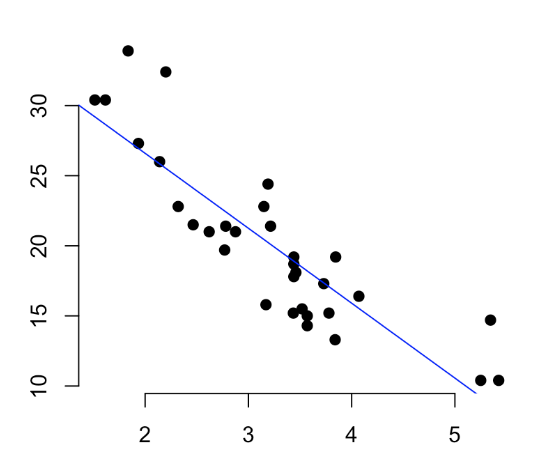
\includegraphics[height=0.4\textheight, keepaspectratio, width=0.9\textwidth]{Sources/scatter-plot-line.png}
\vfill
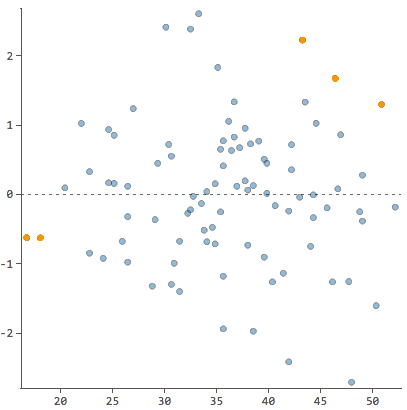
\includegraphics[height=0.4\textheight, keepaspectratio, width=0.9\textwidth]{Sources/scatter-plot-no-relationship.png}
\vfill
\vfill}
\end{column}
\begin{column}{0.5\textwidth}
\vbox to 0.8\textheight{\begin{itemize}
\small
\vfill
\item A scatter plot is a simple way to visualize the relationship between two variables
\vfill
\item If there is a relationship, you will see some defined pattern in the points. This may be somewhat of an upward or downward line (linear relationship) or some other shape such as a U (non-linear relationship).
\vfill
\item If there is no relationship, then there will just be a random cloud of points (lower plot) or a horizontal line.
\end{itemize}}
\end{column}
\end{columns}
\end{frame}
\begin{frame}
\frametitle{Numerically Analyzing the Relationships}
\begin{columns}
\begin{column}{0.5\textwidth}
\vbox to 0.8\textheight{\begin{itemize}
\footnotesize
\vfill
\item The scatter plots help give a broad understanding of the relationship but do not answer the question, how much will my output change if my input changes? E.g. if I earn 10,000 more for a starting salary, how much sooner can I retire?
\vfill
\item Simply increasing the input in your model and checking the output is not enough, because it does not take into account how all the other variables may be changing.
\vfill
\item Multivariate regression is a general tool which is good at answering these kinds of questions, while taking into account all the changing inputs.
\end{itemize}}
\end{column}
\begin{column}{0.5\textwidth}
\vbox to 0.8\textheight{\centering
\vfill
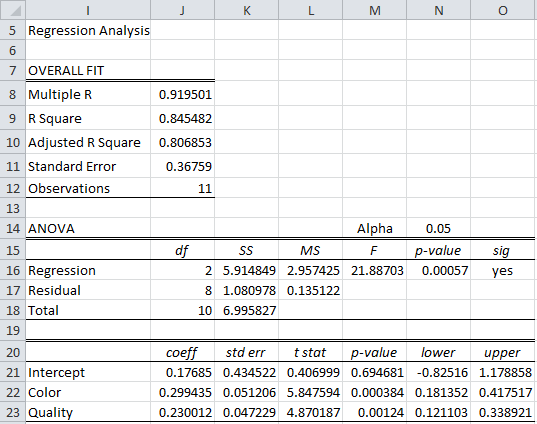
\includegraphics[height=1.0\textheight, keepaspectratio, width=0.9\textwidth]{Sources/excel-multivariate-reg.png}
\vfill
\vfill}
\end{column}
\end{columns}
\end{frame}
\begin{frame}
\frametitle{How to use Multivariate Regression}
\begin{itemize}
\small
\vfill
\item The coefficient in a multivariate regression represents how much the outcome variable changes with a one unit change in the input variable.
\vfill
\item E.g. a coefficient of -.0002 on starting salary in explaining years to retirement would mean that a \$1 increase in starting salary is associated with a decrease in years to retirement by .0002 years, or a \$10,000 increase in starting salary is associated with a decrease in years to retirement by 2 years.
\vfill
\item All interpretations are "all else constant", meaning that it does not consider relationships between the inputs. E.g. if starting salary is higher because of a good economy, and interest rates are also higher due to the good economy, the starting salary coefficient is not taking into account the increase in interest rates.
\vfill
\item Be careful about units. If you use decimals for percentages, you will need to multiply or divide by 100 to get the effect in percentages.
\end{itemize}
\end{frame}
\begin{frame}
\frametitle{Adding Monte Carlo Simulation to a Formal Model}
{
\setbeamercolor{block title}{bg=darkgreen}
\begin{block}{Dynamic Salary Retirement with Monte Carlo}
\begin{itemize}
\item I will now go through adding a Monte Carlo simulation to the Dynamic Salary Retirement Model in Python
\item The completed example is in Examples > Monte Carlo > Python
\end{itemize}
\end{block}
}
\end{frame}
\begin{frame}
\frametitle{Monte Carlo Python Lab, Level 1}
{
\setbeamercolor{block title}{bg=violet}
\begin{block}{Monte Carlo Simulation of Python Models, Level 1}
\begin{enumerate}
\item Work off of your existing Project 1 Python model
\item You are concerned the NPV could be heavily affected by changes in the interest rate. Instead of fixing it, draw it from a normal distribution with mean of 7\% and standard deviation of 2\%.
\item Run the model 10,000 times and collect the years to retirement results. Visualize the results. Create a table of probabilities and the minimum NPV we could expect with that probability. Output the chance that the NPV will be more than \$400,000,000.
\end{enumerate}
\vfill
\begin{tabular*}{\textwidth}{@{\extracolsep{\fill}}ccc}
\toprule
\hfill & Level 2: Slide \textcolor{blue}{\underline{\ref{labs:monte-carlo-python-lab-2}}} & \hfill\\

\end{tabular*}
\end{block}
}
\label{labs:monte-carlo-python-lab-1}
\end{frame}
\end{section}
\begin{section}[Excel MC]{Monte Carlo Simulation in Excel}
\begin{frame}
\frametitle{How is it Different Running MC in Excel?}
\begin{itemize}
\item In pure Excel, it is much more difficult to run a Monte Carlo Simulation
\vfill
\item Without going to VBA, typically the only way is to use a data table
\vfill
\item A data table can be used in situations where you only want to have one or two inputs varying at once. Just generate the random inputs and use them as the axes of the data table
\vfill
\item If you want to vary more than two inputs, VBA or Python would be required
\vfill
\item There are also add-ons that accomplish this but they are usually not free
\end{itemize}
\end{frame}
\begin{frame}
\frametitle{Monte Carlo in Excel with More than Two Variables}
\begin{itemize}
\item The process for Monte Carlo Simulation which works for any number of variables is very similar to what we were doing in Python.
\vfill
\item We are still just changing the inputs, running the model, and storing the outputs from each run
\vfill
\item Using
\texttt{xlwings}
from Python code we can change and retrieve the values of cells
\vfill
\item This allows us to change inputs, run the model, and store outputs, just as in Python, but running our Excel model.
\vfill
\item We can either analyze the outputs in Python or output them back to Excel for analysis
\end{itemize}
\end{frame}
\begin{frame}
\frametitle{Monte Carlo Excel Retirement Model}
{
\setbeamercolor{block title}{bg=darkgreen}
\begin{block}{Using \texttt{xlwings} to Run Monte Carlo Simulations}
\begin{itemize}
\item Go to Canvas and download the "Dynamic Salary Retirement Model.xlsx" and "Excel Monte Carlo.ipynb" from Examples > Monte Carlo > Excel
\item Open up the Jupyter notebook and follow along with me
\item The completed Excel model is also there in case you lose track. Visualizations were added after running the Jupyter notebook on the original Excel model.
\end{itemize}
\end{block}
}
\end{frame}
\begin{frame}
\frametitle{Monte Carlo Excel Lab, Level 1}
{
\setbeamercolor{block title}{bg=violet}
\begin{block}{Monte Carlo Simulation of Excel Models, Level 1}
\begin{enumerate}
\item You will be running Monte Carlo simulations on your existing Excel model from Project 1
\item You are concerned that your estimate for the number of phones that will be sold is incorrect. 
\item The number of phones should instead be drawn from a normal distribution with mean 100,000 and standard deviation of 20,000.
\item Estimate the model 1,000 times and output the results back to Excel
\item In Excel, visualize the results.  Create a table of probabilities and the minimum NPV we could expect with that probability. Output the chance that the NPV will be more than \$800,000,000.
\end{enumerate}
\vfill
\begin{tabular*}{\textwidth}{@{\extracolsep{\fill}}ccc}
\toprule
\hfill & Level 2: Slide \textcolor{blue}{\underline{\ref{labs:monte-carlo-excel-lab-2}}} & \hfill\\

\end{tabular*}
\end{block}
}
\label{labs:monte-carlo-excel-lab-1}
\end{frame}
\end{section}
\appendix
\newcounter{finalframe}
\setcounter{finalframe}{\value{framenumber}}
\begin{frame}
\frametitle{Intro Monte Carlo Lab, Level 2}
{
\setbeamercolor{block title}{bg=violet}
\begin{block}{Monte Carlo Simulation of DDM, Level 2}
\begin{enumerate}
\item Continue from the first lab exercise
\item Now you are also concerned you have mis-estimated the cost of capital. So now use a mean of 9\% and standard deviation of 2\%, in addition to varying the growth
\item Visualize and summarize the resulting probability distribution of the price
\item Be careful as in some cases, the drawn cost of capital will be lower than the drawn growth rate, which breaks the DDM. You will need to modify your logic to throw out these cases.
\end{enumerate}
\vfill
\begin{tabular*}{\textwidth}{@{\extracolsep{\fill}}ccc}
\toprule
\hfill & Level 1: Slide \textcolor{blue}{\underline{\ref{labs:intro-monte-carlo-lab-1}}} & \hfill\\

\end{tabular*}
\end{block}
}
\label{labs:intro-monte-carlo-lab-2}
\end{frame}
\begin{frame}
\frametitle{Monte Carlo Python Lab, Level 2}
{
\setbeamercolor{block title}{bg=violet}
\begin{block}{Monte Carlo Simulation of Python Models, Level 2}
\begin{enumerate}
\item Continue from the first lab exercise. Now you are also concerned that your assembly line will not be as efficient amd so the number of phones per machine will be lower. So draw that from a normal distribution with mean 100,000 and standard deviation of 20,000. 
\item As you run the model, also store what were the interest and number of phones corresponding to the NPV. You want to see which has a greater impact on the NPV: interest or number of phones. Visualize the relationship between interest and NPV, and the relationship between beginning salary and NPV. Also run a regression to quantitatively determine which has a greater effect.
\end{enumerate}
\vfill
\begin{tabular*}{\textwidth}{@{\extracolsep{\fill}}ccc}
\toprule
\hfill & Level 1: Slide \textcolor{blue}{\underline{\ref{labs:monte-carlo-python-lab-1}}} & \hfill\\

\end{tabular*}
\end{block}
}
\label{labs:monte-carlo-python-lab-2}
\end{frame}
\begin{frame}
\frametitle{Monte Carlo Excel Lab, Level 2}
{
\setbeamercolor{block title}{bg=violet}
\begin{block}{Monte Carlo Simulation of Excel Models, Level 2}
\begin{enumerate}
\item Continue from the first lab exercise. Now you are also concerned that there is varying quality in the machines, so they may have a different lifespan. Draw that from a normal distribution with mean 10 years and standard deviation of 2 years.
\item As you run the model, also store what were the number of phones and machine life corresponding to the NPV, all in Excel. You want to see which has a greater impact on the NPV: number of phones or machine life. Visualize the relationship between number of phones and NPV, and the relationship between beginning machine life and NPV. Try to determine which has a greater effect.
\end{enumerate}
\vfill
\begin{tabular*}{\textwidth}{@{\extracolsep{\fill}}ccc}
\toprule
\hfill & Level 1: Slide \textcolor{blue}{\underline{\ref{labs:monte-carlo-excel-lab-1}}} & \hfill\\

\end{tabular*}
\end{block}
}
\label{labs:monte-carlo-excel-lab-2}
\end{frame}
\setcounter{framenumber}{\value{finalframe}}
\end{document}